\documentclass[12pt, a4paper]{article}
\usepackage[latin2]{inputenc}
\usepackage{graphicx}
\usepackage{ulem}
\begin{document}
docx2tex

Kriszti�n P�cza, Mih�ly Bicz�, Zolt�n Porkol�b

E�tv�s Lor�nd University, Fac. of Informatics, Dept. of Programming 
Lang. and Compilers, P�zm�ny P�ter s�t�ny 1/c. H-1117, Budapest, Hungary 


kpocza@kpocza.net, mihaly.biczo@t-online.hu, gsd@elte.hu 

\textbf{Abstract}

This paper has been originally written in Word 2007 and then converted 
to TeX using docx2tex. Docx2tex is a small application that uses 
standard technologies to help users of Word 2007 to publish scientific 
publications to conferences easier where typography merits and only 
papers produced by TeX are accepted. Docx2tex is an open source and free 
application that is accessible and extensible by everyone.

\section{Introduction}There are two general methods to produce human 
readable and printable digital documents:

\newcounter{numberedCntA}
\begin{enumerate}
\item Use some WYSIWYG word processor
\item Use some typesetting system
\setcounter{numberedCntA}{\theenumi}
\end{enumerate}
Each of them has its own advantages and disadvantages therefore each of 
them has many use cases where one is better than the other and vice 
versa.

WYSIWYG is the acronym for \textit{What You See Is What You Get} that 
originates from the late '70. WYSIWYG editors are mostly used by 
everyday computer users whose aim is to produce good looking documents 
fast and exploit the rich formatting capabilities of such systems. This 
type of editors, word processors ensures that the printed out version 
of the document will be the same as the visible document on screen while 
editing. The first WYSIWYG word processor called Bravo was created at 
Xerox by Charles Simonyi who originates from Hungary, invented 
intentional programming and visited the space in 2007. In 1981 Simonyi 
left Xerox and joined Microsoft where he created Microsoft Word the 
first and to this day most popular word processor. Word is capable to 
produce simple and also complex documents even with lot of mathematical 
symbols.

Typesetting is the process of putting characters of different type in 
their correct place on the paper or screen. The aim of typesetting 
systems is to create high quality output of materials that may contain 
complex mathematical formulas and complex figures. Before the electronic 
typesetting systems the printed materials were produced by compositors 
who worked by hand or by special machines. The electronic typesetting 
systems follow this way and produce high quality, device independent 
output. The most popular typesetting system is TeX created by Donald E. 
Knuth that is mainly used by researchers and by anyone whose aim is to 
achieve the best quality printout. The users of TeX use a special and 
extensible DSL (Domain Specific Language) that was designed to solve 
complex typesetting problems or even produce many-hundred-page books.

There is a big gap between these systems because each takes aim at 
different result. To converge them there are some commercial and 
non-commercial applications that support converting between Word or 
other WHYSIWYG formats and TeX. Converting from WHYSIWYG (Word) formats 
to TeX has more reason for existence because many users edit the 
original text in Word and then convert it to TeX to ensure professional 
printout. 

The problems with present applications supporting this scenario are the 
following:

\newcounter{numberedCntB}
\begin{enumerate}
\item They are not free
\item Has some limitations (running times or page limit) when not 
purchased 
\item Support only the old, closed Word document format (DOC and not 
DOCX)
\item Use the COM API of Word to process documents that makes them 
complex
\setcounter{numberedCntB}{\theenumi}
\end{enumerate}
In this paper we present an open source and free solution that is 
capable of handling the new and open Word 2007 DOCX format natively 
using standard technologies without leveraging the COM API of Word and 
without installing Word. We present the current features and some 
further development directions.

\section{The Technology}In this section we will enumerate and then 
shortly review the technologies that are used in docx2tex and show how 
they cooperate.

The used technologies are the following:

\newcounter{numberedCntC}
\begin{enumerate}
\item Standard XML and XSLT technologies
\item Office Open XML (ECMA 376 Standard), the default format of Word 
2007 - OOXML
\item Microsoft .NET 3.0 (CLI is ECMA 335 Standard)
\item ImageMagick to convert images 
\setcounter{numberedCntC}{\theenumi}
\end{enumerate}
OOXML files are XML and media files compressed using ZIP together. 
Docx2tex uses Microsoft .NET 3.0 to open and unzip OOXML Word 2007 DOCX 
documents. Microsoft .NET 3.0 has some special classes in the \textit{
System.IO.Packaging} namespace that facilitate opening and unzipping 
OOXML files and abstract the contained XML and media files as packages. 
The most important component of docx2tex is a set of XSLT files that 
leverages the conversation from XML files to TeX. When an image 
reference is found in the XML while XSL transformation a .NET function 
is called that uses ImageMagick to produce EPS files from the original 
image files. EPS files can be then simply embedded in TeX documents.

The previous description is illustrated by the following UML sequence 
diagram:

\begin{figure}[h]
\centering
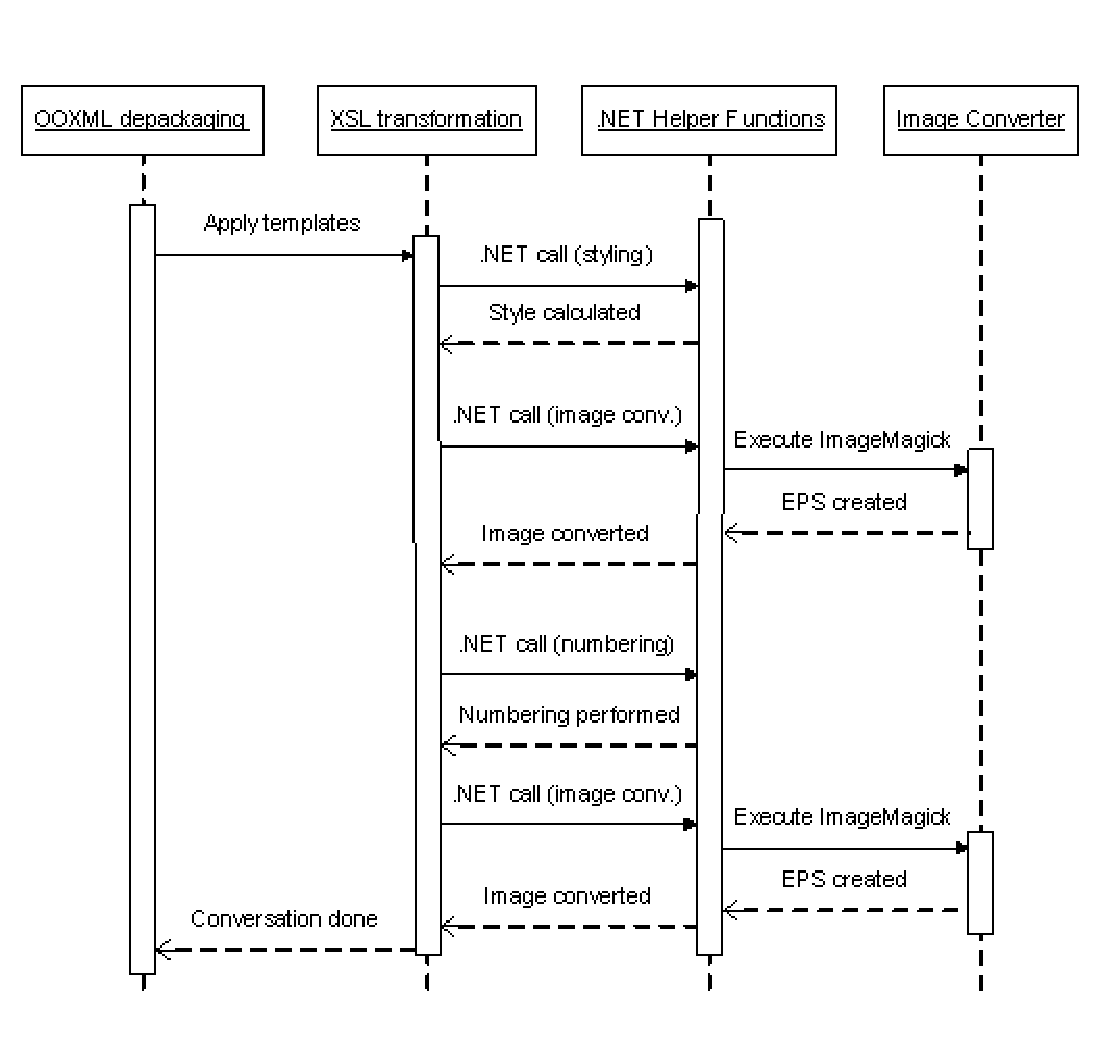
\includegraphics[width=383.15pt,height=369.4pt]{media/image1.eps}
\caption{Figure : UML}
\end{figure}



\section{Features of Docx2tex}In this section we first present the 
supported and then the unsupported features of docx2tex.

\subsection{Supported Features}Docx2tex supports the following 
features of Word 2007 and Tex:

\newcounter{numberedCntD}
\begin{enumerate}
\item Normal text
\item Italic, bold, underlined, stroked, small capitals, ...
\item Left, right, center aligned text
\item Headings - sections (3 levels)
\item Simple tables
\item Line and page breaks 
\item Numbered and bulleted lists
\item Multilevel lists and continuous numbered lists
\item Figure, table and listing captions
\item Cross reference to captions and headings
\item Image conversion from various formats (incl. PNG and JPEG) to EPS
\item Substitution of special characters (e.g. $\backslash$, \#, \{, \}, 
$[$, $]$, \\%, \&, \~, ...)
\setcounter{numberedCntD}{\theenumi}
\end{enumerate}
It supports normal and special text styles and also text alignments but 
does not support different fonts. We support Heading1, Heading2, and 
Heading3 which convert to $\backslash$section, $\backslash$subsection, 
and $\backslash$subsubsection respectively. Only simple, left aligned 
tables are supported. Both numbered and bulleted lists are supported, 
moreover these lists can be embedded together and continuous lists are 
also supported using the $\backslash$setcounter, the $\backslash$enumi, 
and the $\backslash$theenumi commands. Figure, table and listings 
captions are recognized and we support referencing them together with 
heading references also. Image references are resolved and the images 
(mainly PNG and JPEG) embedded in the OOXML documents are converted to 
EPS. The width and height properties are queried and the same 
properties are used in the resulting TeX documents. Some special TeX 
characters are also resolved and escaped in the resulting TeX document.

\subsection{Unsupported Features}We plan to add support for Word 2007 
Equations and Drawings that can be converted to TeX mathematical 
formulas and Fig respectively. Both of them is described in XML format 
therefore our standard solution, XSL transformations can be used.

\section{A Complex Example}In this section we will show a complex 
example broken into parts that can show the most important features of 
docx2tex.

\subsection{The Structure of the OOXML Zip Package}First unzip the 
contents of our OOXML Word 2007 document to a directory and get a 
directory listing recursively:

\begin{verbatim}
PS C:\Phd\conferences\2008_3_tex\example.docx> ls -Recu |% {$_.FullName.SubString(30)}
example.docx\customXml
example.docx\docProps
example.docx\word
example.docx\_rels
example.docx\[Content_Types].xml
example.docx\customXml\_rels
example.docx\customXml\item1.xml
example.docx\customXml\itemProps1.xml
example.docx\customXml\_rels\item1.xml.rels
example.docx\docProps\app.xml
example.docx\docProps\core.xml
example.docx\word\media
example.docx\word\theme
example.docx\word\_rels
example.docx\word\document.xml
example.docx\word\fontTable.xml
example.docx\word\numbering.xml
example.docx\word\settings.xml
example.docx\word\styles.xml
example.docx\word\webSettings.xml
example.docx\word\media\image1.jpeg
example.docx\word\theme\theme1.xml
example.docx\word\_rels\document.xml.rels
example.docx\_rels\.rels
\end{verbatim}
The most important part is the document.xml that contains the document 
itself and references to outer items. The numbering.xml specify the 
style of the numbered or bulleted lists contained in the document.xml. 
The styles.xml specify information about the styles used in the 
document. Under the media directory the embedded images can be found 
(image1.jpeg in our example).

\subsection{Structure of the Document}The text in document.xml is 
grouped in paragraphs. Every segment of the document is a paragraph 
(normal text, heading texts, images, etc.) except for some special 
elements like tables.

Consider the following example sentence: This is a \textit{$^{sentence
}$}\textbf{\textit{ that}} \underline{contains} text \textbf{
\textit{\underline{with}}} \sout{different} $_{formatting}$.

\begin{verbatim}
This sentence is described as the following in OOXML format:
<w:p w:rsidR="004F5706" w:rsidRDefault="004F5706" w:rsidP="004F5706">
  <w:r w:rsidRPr="0030655B">
    <w:t xml:space="preserve">This is a </w:t>
  </w:r>
  <w:r w:rsidRPr="0030655B">
    <w:rPr>
      <w:i/>
      <w:vertAlign w:val="superscript"/>
    </w:rPr>
    <w:t>sentence</w:t>
  </w:r>
  <w:r w:rsidRPr="0030655B">
    <w:rPr>
      <w:b/>
      <w:i/>
    </w:rPr>
    <w:t xml:space="preserve"> that</w:t>
  </w:r>
  <w:r w:rsidRPr="0030655B">
    <w:t xml:space="preserve"> </w:t>
  </w:r>
  <w:r w:rsidRPr="0030655B">
    <w:rPr>
      <w:u w:val="single"/>
    </w:rPr>
    <w:t>contains</w:t>
  </w:r>
  <w:r w:rsidRPr="0030655B">
    <w:t xml:space="preserve"> text </w:t>
  </w:r>
  <w:r w:rsidRPr="0030655B">
    <w:rPr>
      <w:b/>
      <w:i/>
      <w:u w:val="single"/>
    </w:rPr>
    <w:t>with</w:t>
  </w:r>
  <w:r w:rsidRPr="0030655B">
    <w:t xml:space="preserve"> </w:t>
  </w:r>
  <w:r w:rsidRPr="0030655B">
    <w:rPr>
      <w:strike/>
    </w:rPr>
    <w:t>different</w:t>
  </w:r>
  <w:r w:rsidRPr="0030655B">
    <w:t xml:space="preserve"> </w:t>
  </w:r>
  <w:r w:rsidRPr="0030655B">
    <w:rPr>
      <w:vertAlign w:val="subscript"/>
    </w:rPr>
    <w:t>formatting</w:t>
  </w:r>
  <w:r w:rsidRPr="0030655B">
    <w:t>.</w:t>
  </w:r>
</w:p>
\end{verbatim}


XML node \textit{$<$w:p$>$} and \textit{$<$/w:p$>$} encloses a 
paragraph while \textit{$<$w:r$>$} and \textit{$<$/w:r$>$ } encloses 
a run. A run contains a range of text (between \textit{$<$w:t$>$} and 
\textit{$<$/w:t$>$}) and may contain some formatting between \textit{
$<$w:rPr$>$} and \textit{$<$/w:rPr$>$} (\textit{$<$w:b/$>$} means 
bold, while \textit{$<$w:i/$>$} means italic font style).

The TeX output generated by docx2tex of the previous sentence looks the 
following:

\begin{verbatim}
This is a \textit{$^{sentence}$}\textbf{\textit{ that}} \underline{contains} text \textbf{\textit{\underline{with}}} \sout{different} $_{formatting}$.
\end{verbatim}


Another important feature of docx2tex is handling headings. Consider the 
following OOXML fragment:

\begin{verbatim}
<w:p w:rsidR="004F5706" w:rsidRPr="0030655B" w:rsidRDefault="004F5706" w:rsidP="000136DF">
  <w:pPr>
    <w:pStyle w:val="Heading1"/>
  </w:pPr>
  <w:bookmarkStart w:id="0" w:name="_Ref186547407"/>
  <w:r w:rsidRPr="0030655B">
    <w:t>Heading text</w:t>
  </w:r>
  <w:bookmarkEnd w:id="0"/>
</w:p>
\end{verbatim}


The \textit{$<$w:pStyle w:val="Heading1" /$>$} node specifies that a 
first level heading begins, while the contained \textit{
$<$w:bookmarkStart w:id="0" w:name="\_Ref186547407" /$>$ }node 
specifies a unique internal reference (bookmark) to the heading that can 
be cross-references from any part of the document. 

The generated TeX output is the following:

\begin{verbatim}
\section{Heading text}\label{section:_Ref186547407}
\end{verbatim}


Images are described in OOXML in a very loose way, there is no space to 
show the original XML fragment. Instead we show only the generated TeX 
code:

\begin{verbatim}
\begin{figure}[h]
\centering
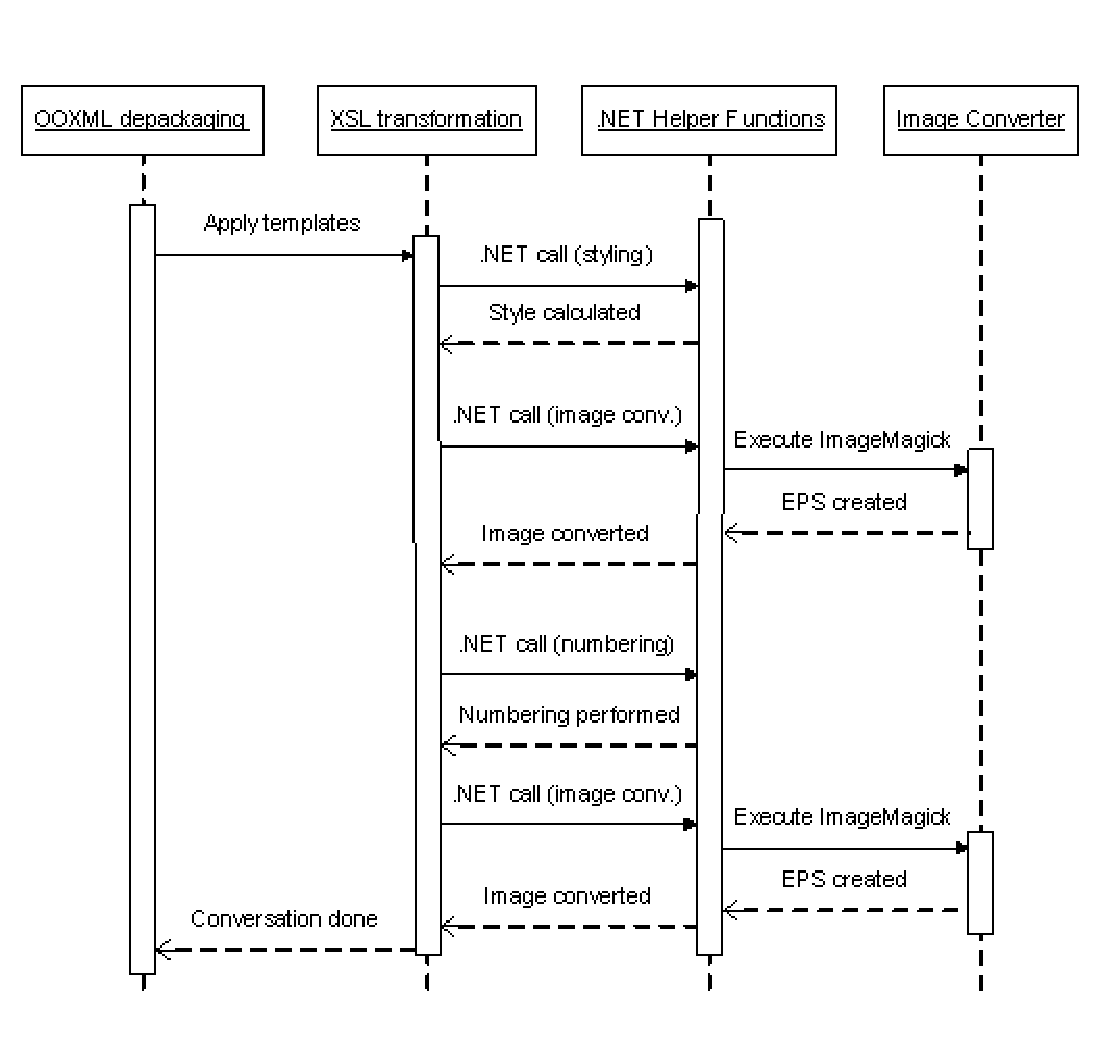
\includegraphics[width=10.52cm,height=8.41cm]{media/image1.eps}
\caption{\label{figure:_Ref186544261}: Figure caption}
\end{figure}
\end{verbatim}


The image is centered and the width and the height of the image are 
preserved. Image1.jpeg was converted to image1.eps the files was saved 
in the media subdirectory. When the image has a caption then it is also 
added to the output so that it can be referenced.

Reference to the previous figure is described in OOXML in the following 
form:

\begin{verbatim}
<w:p w:rsidR="004F5706" w:rsidRPr="0030655B" w:rsidRDefault="004F5706" w:rsidP="004F5706">
  <w:pPr>
    <w:keepNext/>
  </w:pPr>
  <w:r w:rsidRPr="0030655B">
    <w:t xml:space="preserve">Reference to the figure: </w:t>
  </w:r>
  <w:r w:rsidR="007A289D">
    <w:fldChar w:fldCharType="begin"/>
  </w:r>
  <w:r w:rsidR="006B4DA8">
    <w:instrText xml:space="preserve"> REF _Ref186544261 \h </w:instrText>
  </w:r>
  <w:r w:rsidR="007A289D">
    <w:fldChar w:fldCharType="separate"/>
  </w:r>
  <w:r w:rsidR="006B4DA8">
    <w:t xml:space="preserve">Figure </w:t>
  </w:r>
  <w:r w:rsidR="006B4DA8">
    <w:rPr>
      <w:noProof/>
    </w:rPr>
    <w:t>1</w:t>
  </w:r>
  <w:r w:rsidR="007A289D">
    <w:fldChar w:fldCharType="end"/>
  </w:r>
</w:p>
\end{verbatim}
The generated TeX code is as simple as (it can be seen the \textit{
Figure 1} text has been omitted from the output): 

Reference to the figure: $\backslash$ref\{figure:\_Ref186544261\}.

The first item of a numbered list looks the following (\textit{1. 
First} can be seen on the screen):

\begin{verbatim}
<w:p w:rsidR="004F5706" w:rsidRPr="0030655B" w:rsidRDefault="004F5706" w:rsidP="004F5706">
  <w:pPr>
    <w:pStyle w:val="ListParagraph"/>
    <w:keepNext/>
    <w:numPr>
      <w:ilvl w:val="0"/>
      <w:numId w:val="1"/>
    </w:numPr>
  </w:pPr>
  <w:r w:rsidRPr="0030655B">
    <w:t>First</w:t>
  </w:r>
</w:p>
\end{verbatim}


The nodes embedded into \textit{$<$w:numPr$>$} and \textit{
$<$/w:numPr$>$} nodes specify the we are using the numbering style 1 on 
level 0. The corresponding numbering parameters are defined in 
numbering.xml that is processed by docx2tex. The above element is the 
part of a complex multilevel numbered list:



\begin{verbatim}
\newcounter{numberedCntA}
\begin{enumerate}
\item First
\item Second
\item Third
\begin{enumerate}
\item First
\item Second
\item Third
\end{enumerate}
\item Fourth
\setcounter{numberedCntA}{\theenumi}
\end{enumerate}
\end{verbatim}


When we want to continue the previous list $\backslash$se
tcounter\{enumi\}\{$\backslash$thenumberedCntA\} have to be called 
after the certain $\backslash$begin\{enumerate\} that continues the list
.



There is no space to show the OOXML version of a simple table that has 
four cells. The generated TeX output is the following:



\begin{verbatim}
\begin{tabular}{|l|l|}
\hline
1 & 2 \\
\hline
3 & 4 \\
\hline
\end{tabular}
\caption{\label{table:_Ref186545972}: caption}
\end{table}
\end{verbatim}


Consider the following set of special characters: $<$$>$ as'q ...\# 
$\backslash$ \{ \} \\% \~ \_ \^{} \& \$ "\," \\
These are described in OOXML in the following form:

\begin{verbatim}
<w:p w:rsidR="00AB630B" w:rsidRDefault="00AB630B" w:rsidP="00AB630B">
  <w:r>
    <w:t xml:space="preserve">&lt;&gt; </w:t>
  </w:r>
  <w:proofErr w:type="spellStart"/>
  <w:r>
    <w:t>as'q</w:t>
  </w:r>
  <w:proofErr w:type="spellEnd"/>
  <w:r>
    <w:t xml:space="preserve"> ...# \ { } </w:t>
  </w:r>
  <w:proofErr w:type="gramStart"/>
  <w:r>
    <w:t>%  ~</w:t>
  </w:r>
  <w:proofErr w:type="gramEnd"/>
  <w:r>
    <w:t xml:space="preserve"> _ ^ &amp; $ ""</w:t>
  </w:r>
</w:p>
\end{verbatim}
The resulting TeX code is: 
\$$<$\$\$$>$\$ 
as'q ...$\backslash$\# 
\$$\backslash$backslash\$ $\backslash$\{ 
$\backslash$\} $\backslash$\\% $\backslash$\~ $\backslash$\_ 
$\backslash$\^{} $\backslash$\& \$ "$\backslash$,"



\end{document}
